\documentclass[
	a4paper,
	oneside,
	DIV = 12,
	fontsize = 13pt,
	headings = normal,
]{scrartcl}

%%% Page geometry and precise margins
\usepackage[
	pass,
	left   = 20mm,
	top    = 15mm,
	right  = 10mm,
	bottom = 15mm,
]{geometry}
%%%

%%% Length calculations
\usepackage{calc}
%%%

%%% Support for color
\usepackage{xcolor}
\definecolor{lightblue}{HTML}{03A9F4}
\definecolor{red}{HTML}{F44336}
%%%

%%% Including graphics
\usepackage{graphicx}
%%%

%%% Font selection
\usepackage{fontspec}

\setromanfont{STIX Two Text}[
	SmallCapsFeatures = {LetterSpace = 5},
]

\setsansfont{IBM Plex Sans}[
	Scale = MatchUppercase,
]

\setmonofont{IBM Plex Mono}[
	Scale = MatchUppercase,
]
%%%

%%% Math typesetting
\usepackage{amsmath}

\usepackage{unicode-math}
\setmathfont{STIX Two Math}
%%%

%%% List settings
\usepackage{enumitem}
\setlist[enumerate]{
	label*      = {\arabic*.},
	leftmargin  = *,
	labelindent = \parindent,
	topsep      = 1\baselineskip,
	parsep      = 0\baselineskip,
	itemsep     = 1\baselineskip,
}

\setlist[itemize]{
	label       = {—},
	leftmargin  = *,
	labelindent = \parindent,
	topsep      = 1\baselineskip,
	parsep      = 0\baselineskip,
	itemsep     = 1\baselineskip,
}

\setlist[description]{
	font        = {\rmfamily\upshape\bfseries},
	topsep      = 1\baselineskip,
	parsep      = 0\baselineskip,
	itemsep     = 0\baselineskip,
}

%%%

%%% Structural elements typesetting
\setkomafont{pagenumber}{\rmfamily}
\setkomafont{disposition}{\rmfamily\bfseries}

% Sectioning
\RedeclareSectionCommand[
	beforeskip = -1\baselineskip,
	afterskip  = 1\baselineskip,
	font       = {\normalsize\bfseries\scshape},
]{section}

\RedeclareSectionCommand[
	beforeskip = -1\baselineskip,
	afterskip  = 1\baselineskip,
	font       = {\normalsize\bfseries},
]{subsection}

\RedeclareSectionCommand[
	beforeskip = -1\baselineskip,
	afterskip  = 1\baselineskip,
	font       = {\normalsize\bfseries},
]{subsubsection}
%%%

%%% Typographic enhancements
\usepackage{microtype}
%%%

%%% Language-specific settings
\usepackage{polyglossia}
\setmainlanguage{ukrainian}
\setotherlanguages{english, russian}
%%%

%%% Captions
\usepackage{caption}
\usepackage{subcaption}

%\DeclareCaptionLabelFormat{closing}{#2)}
%\captionsetup[subtable]{labelformat = closing}

%\captionsetup[subfigure]{labelformat = closing}

\captionsetup[table]{
	aboveskip = 0\baselineskip,
	belowskip = 1\baselineskip,
}

\captionsetup[figure]{
	aboveskip = 1\baselineskip,
	belowskip = 0\baselineskip,
}

\captionsetup[subfigure]{
	aboveskip = 0.25\baselineskip,
	belowskip = 0\baselineskip,
}

\captionsetup[subfigure]{
	labelformat = simple,
	labelformat = brace,
}
%%%

%%% Table typesetting
\usepackage{booktabs}
\usepackage{longtable}

\usepackage{multirow}

\usepackage{array}
\newcolumntype{v}[1]{>{\raggedright\arraybackslash\hspace{0pt}}p{#1}}
\newcolumntype{b}[1]{>{\centering\arraybackslash\hspace{0pt}}p{#1}}
\newcolumntype{n}[1]{>{\raggedleft\arraybackslash\hspace{0pt}}p{#1}}
%%%

%%% Dingbats
\usepackage{pifont}
%%%

%%% TikZ
\usepackage{tikz}
%%%

%%% Links and hyperreferences
\usepackage{hyperref}
\hypersetup{
	bookmarksnumbered = true,
	colorlinks      = false,
	linkbordercolor = red,
	urlbordercolor  = lightblue,
	pdfborderstyle  = {/S/U/W 1.5},
}
%%%

%%% Length adjustments
% Set baselineskip to ~15pt, default is 14.5pt
% \linespread{1.034483}
% \linespread{1.068966} % ~15.5pt
\setlength{\emergencystretch}{1em}
\setlength{\parindent}{1.5em}
\newlength{\gridunitwidth}
\setlength{\gridunitwidth}{\textwidth / 12}
\setlength{\floatsep}{1\baselineskip}
\setlength{\intextsep}{1\baselineskip}
\setlength{\textfloatsep}{1\baselineskip}
%%%

%%% Custom commands
\newcommand{\allcaps}[1]{{\addfontfeatures{LetterSpace = 5}#1}}
\newcommand{\progname}[1]{\texttt{#1}}

\newcommand{\CheckMark}{\ding{51}}
\newcommand{\Mytextrightarrow}{$\rightarrow$\hspace{0.25em}}

\newcommand{\filename}[1]{\texttt{#1}}
%%%

%%% Make typography adhere to made-up standards
\PolyglossiaSetup{ukrainian}{indentfirst = true}

% Sectioning
\RedeclareSectionCommand[
	beforeskip = -0sp,
	afterskip  = 1sp,
	indent     = 12.5mm,
	font       = {\normalsize\bfseries},
]{section}

\RedeclareSectionCommand[
	beforeskip = -0sp,
	afterskip  = 1sp,
	indent     = 12.5mm,
	font       = {\normalsize\bfseries},
]{subsection}

\RedeclareSectionCommand[
	beforeskip = -0sp,
	afterskip  = 1sp,
	indent     = 12.5mm,
	font       = {\normalsize\bfseries},
]{subsubsection}

\setlength{\parindent}{12.5mm}

\usepackage{leading}
\leading{21pt}

%%%

\begin{document}
	\newgeometry{
		left   = 20mm,
		top    = 15mm,
		right  = 10mm,
		bottom = 15mm,
		footskip = \baselineskip, % reduce footer vertical skip so page numbers are visible
	}
\setlength{\gridunitwidth}{\textwidth / 12}
	\begin{titlepage}
		\begin{center}
			Міністерство освіти і науки України\\
			Національний авіаційний університет\\
			Навчально-науковий інститут комп'ютерних інформаційних технологій\\
			Кафедра комп'ютеризованих систем управління

			\vspace{\fill}
				Лабораторна робота №6\\
				з~дисципліни «Діагностика та~експлуатація комп'ютера»\\
				на~тему «Командний рядок \textenglish{Windows XP}»\\

			\vspace{\fill}

			\begin{flushright}
				Виконав:\\
				студент \allcaps{ННІКІТ}\\
				групи СП-325\\
				Клокун В.\,Д.\\
				Перевірив:\\
				Масловський Б.\,Г.
			\end{flushright}

			Київ 2018
		\end{center}
	\end{titlepage}

	\section{Ціль роботи}
		Ознайомлення з~командами командного рядку та отримання практичних навичок роботи з ними.

	% \section{Короткі теоретичні відомості}

	\section{Хід роботи}
		Запускаємо командний рядок \textenglish{Windows XP} та починаємо виконувати команди \progname{date, echo, path, popd, pushd, title, type, ver}.

		\subsection{Команда~\progname{date}}
			Команда~\progname{date} призначена для виведення, встановлення та зміни дати~(приклад роботи на рис.~\ref{fig:echo-usage}).

			\begin{figure}[!htbp]
				\centering
				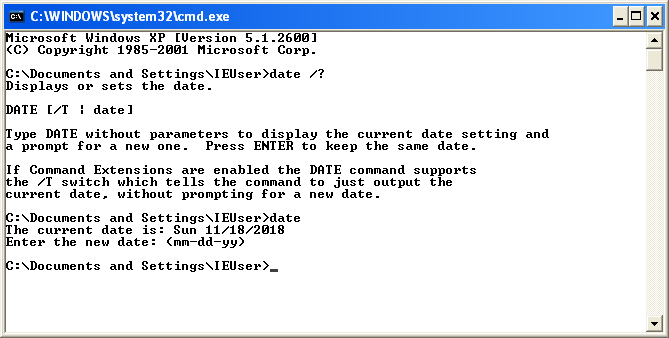
\includegraphics[height = 6\baselineskip]{../01-solution/y03s01-pcdiag-lab-06-p01.png}
				\caption{Приклад роботи команди~\progname{date}}
				\label{fig:date-usage}
			\end{figure}

			Щоб вивести поточну дату, необхідно запустити команду без параметрів. Щоб не змінювати дату, необхідно натиснути клавішу \textenglish{Enter}. Якщо увімкнені розширення командної строки, команда~\progname{date} підтримує параметр~\texttt{/I}, при передачі якого команда не запрошує користувача змінити поточну дату.

		\subsection{Команда~\progname{echo}}
			Команда~\progname{date} призначена для виведення повідомлень, а також ввімкнення та вимкнення повторного виводу введених команд~(приклад роботи на рис.~\ref{fig:echo-usage}).

			\begin{figure}[!htbp]
				\centering
				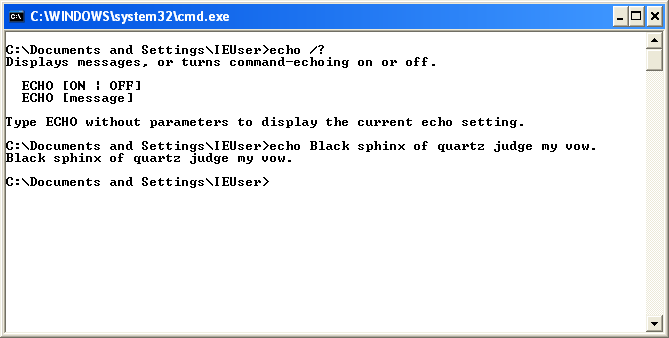
\includegraphics[height = 6\baselineskip]{../01-solution/y03s01-pcdiag-lab-06-p02.png}
				\caption{Приклад роботи команди~\progname{echo}}
				\label{fig:echo-usage}
			\end{figure}

			Щоб вивести поточні налаштування повторного виводу команд, необхідно запустити команду без параметрів. Щоб вивести будь-яке повідомлення, необхідно ввести назву команди та текст бажаного повідомлення і~натиснути клавішу \textenglish{Enter}. 

		\subsection{Команда~\progname{path}}
			Команда~\progname{path} призначена для виведення або зміни шляхів, в яких виконується пошук виконуваних файлів~(приклад роботи на рис.~\ref{fig:path-usage}).

			\begin{figure}[!htbp]
				\centering
				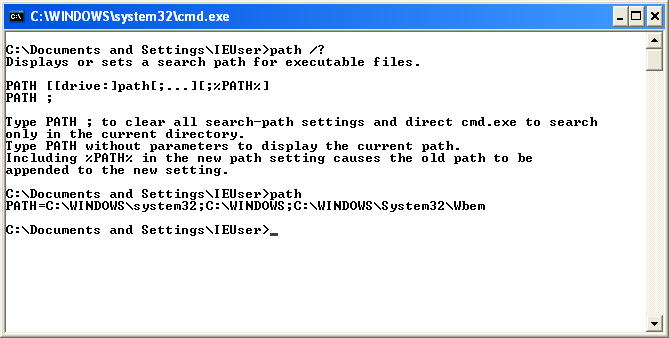
\includegraphics[height = 6\baselineskip]{../01-solution/y03s01-pcdiag-lab-06-p03.png}
				\caption{Приклад роботи команди~\progname{path}}
				\label{fig:path-usage}
			\end{figure}

			Щоб очистити поточні шляхи пошуку виконуваних файлів, необхідно ввести \verb|path ;|. У такому випадку виконувані файли будуть шукатись виключно у поточній директорії.

			Щоб вивести поточні шляхи пошуку виконуваних файлів, необхідно запустити команду без параметрів. Щоб додати певні шляхи до поточного значення, треба використати поточне значення змінної. Наприклад, так:
			\begin{verbatim}
path %PATH%;C:\NewSearchPath\
			\end{verbatim}

		\subsection{Команди~\progname{popd} і~\progname{pushd}}
			Команда~\progname{popd} призначена для збереження місцезнаходження поточної директорії для використання командою~\progname{popd} і подальшого переходу до бажаної директорії. Команда~\progname{popd} повертається до директорії, збереженої командою~\progname{pushd}~(приклад роботи на рис.~\ref{fig:pushd-popd-usage}).

			\begin{figure}[!htbp]
				\centering
				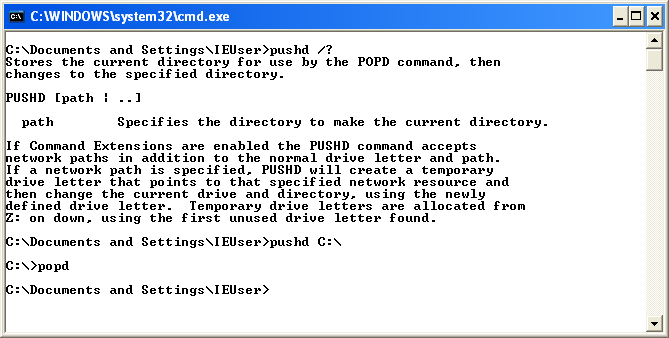
\includegraphics[height = 6\baselineskip]{../01-solution/y03s01-pcdiag-lab-06-p04.png}
				\caption{Приклад роботи команд~\progname{pushd} і~\progname{popd}}
				\label{fig:pushd-popd-usage}
			\end{figure}

			Якщо увімкнені розширення командної строки, окрім звичайних шляхів команда також приймає і мережеві. В такому випадку команда~\progname{pushd} створює тимчасову дискову літеру, ставить її у відповідність бажаному мережевому ресурсу та переходить на його місце, використовуючи щойно створену дискову літеру. Літери виділяються від \textenglish{\texttt{Z:}} у спадному лексичному порядку, використовуючи першу вільну літеру.

		\subsection{Команда~\progname{type}}
			Команда~\progname{type} призначена для виведення змісту одного або декількох текстових файлів~(приклад роботи на рис.~\ref{fig:type-usage}).

			\begin{figure}[!htbp]
				\centering
				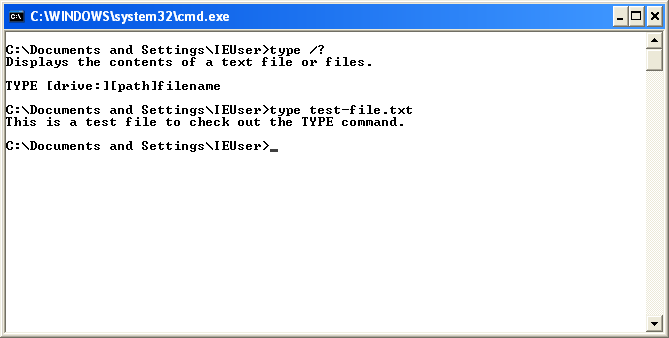
\includegraphics[height = 6\baselineskip]{../01-solution/y03s01-pcdiag-lab-06-p05.png}
				\caption{Приклад роботи команди~\progname{type}}
				\label{fig:type-usage}
			\end{figure}

			Параметрами команди~\progname{type} є будь-яка кількість текстових файлів, зміст яких необхідно вивести.

		\subsection{Команда~\progname{title}}
			Команда~\progname{title} призначена для встановлення заголовку вікна командного рядка~(приклад роботи на рис.~\ref{fig:title-usage}).

			\begin{figure}[!htbp]
				\centering
				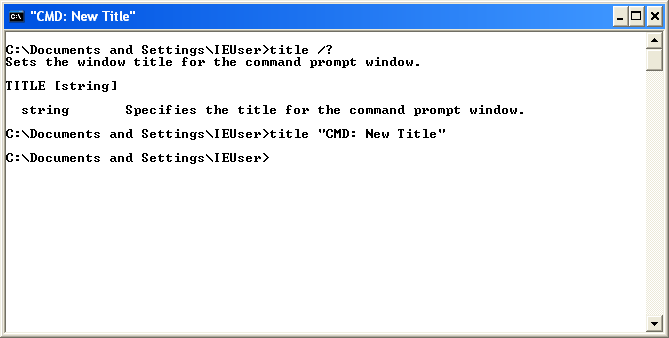
\includegraphics[height = 6\baselineskip]{../01-solution/y03s01-pcdiag-lab-06-p06.png}
				\caption{Приклад роботи команди~\progname{title}}
				\label{fig:title-usage}
			\end{figure}

			Параметрами команди~\progname{title} є рядок, який містить бажаний заголовок вікна командного рядка.

		\subsection{Команда~\progname{ver}}
			Команда~\progname{ver} призначена для виведення поточної версії операційної системи~(приклад роботи на рис.~\ref{fig:ver-usage}).

			\begin{figure}[!htbp]
				\centering
				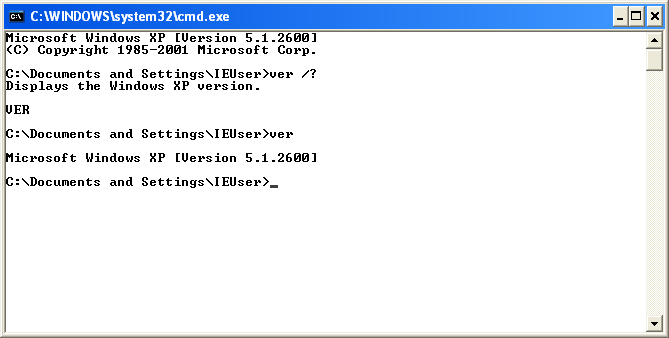
\includegraphics[height = 6\baselineskip]{../01-solution/y03s01-pcdiag-lab-06-p07.png}
				\caption{Приклад роботи команди~\progname{ver}}
				\label{fig:ver-usage}
			\end{figure}

			Команда~\progname{ver} не приймає параметрів, зазвичай запускається без них, а при наданні їх ігнорує.

	\section{Висновки}
		Виконуючи дану лабораторну роботу, ми ознайомились з~командами командного рядку та~отримали практичні навички роботи з~ними.

\end{document}
